\documentclass[tikz,border=2pt]{standalone}
\usepackage{amsmath}
\usepackage{pgfplots}
\pgfplotsset{compat=1.18}
\usetikzlibrary{arrows.meta}
\begin{document}
% Left: x^2 with the chord from a=-1 to b=3; at lambda=1/2 the chord height 5 exceeds f(1)=1 by the gap 4 (strictly convex).
% Right: |x| with the chord from p=0 to q=e_1=1, which lies on the graph (convex, not strictly convex).
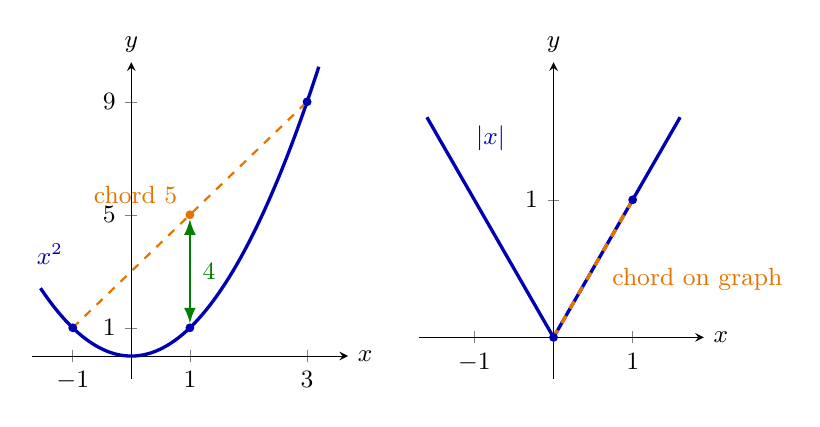
\begin{tikzpicture}[font=\small, >={Latex[length=2mm]}]
  \begin{axis}[
    name=left, axis lines=middle, xmin=-1.7, xmax=3.7, ymin=-0.8, ymax=10.4,
    xtick={-1,1,3}, ytick={1,5,9},
    xlabel={$x$}, ylabel={$y$},
    xlabel style={anchor=west}, ylabel style={anchor=south},
    width=5.6cm, height=5.6cm, clip=false
    ]
    \addplot[blue!70!black, very thick, domain=-1.55:3.2, samples=80] {x^2};
    \node[blue!70!black, anchor=east] at (axis cs:-1.0,3.6) {$x^2$};
    \draw[orange!90!black, thick, dashed] (axis cs:-1,1) -- (axis cs:3,9);
    \fill[blue!70!black] (axis cs:-1,1) circle (1.6pt);
    \fill[blue!70!black] (axis cs:3,9) circle (1.6pt);
    \draw[green!50!black, thick, <->] (axis cs:1,1.15) -- (axis cs:1,4.85);
    \node[green!50!black, anchor=west] at (axis cs:1.05,3) {$4$};
    \fill[orange!90!black] (axis cs:1,5) circle (1.6pt);
    \node[orange!90!black, anchor=south east] at (axis cs:0.95,5.05) {chord $5$};
    \fill[blue!70!black] (axis cs:1,1) circle (1.6pt);
  \end{axis}
  \begin{axis}[
    at={(left.east)}, anchor=west, xshift=0.9cm,
    axis lines=middle, xmin=-1.7, xmax=1.9, ymin=-0.3, ymax=2.0,
    xtick={-1,1}, ytick={1},
    xlabel={$x$}, ylabel={$y$},
    xlabel style={anchor=west}, ylabel style={anchor=south},
    width=5.2cm, height=5.6cm, clip=false
    ]
    \addplot[blue!70!black, very thick] coordinates {(-1.6,1.6) (0,0) (1.6,1.6)};
    \node[blue!70!black, anchor=west] at (axis cs:-1.1,1.45) {$|x|$};
    \draw[orange!90!black, very thick, dashed] (axis cs:0,0) -- (axis cs:1,1);
    \fill[blue!70!black] (axis cs:0,0) circle (1.6pt);
    \fill[blue!70!black] (axis cs:1,1) circle (1.6pt);
    \node[orange!90!black, anchor=west] at (axis cs:0.62,0.42) {chord on graph};
  \end{axis}
\end{tikzpicture}
\end{document}
